\documentclass[a4paper, 14pt]{article}
\usepackage[left=20mm, top=20mm, right=10mm, bottom=20mm]{geometry}

\usepackage[T2A]{fontenc}
\usepackage[utf8]{inputenc}
\usepackage[russian]{babel}

\usepackage{hyphenat}
\hyphenation{ма-те-ма-ти-ка вос-ста-нав-ли-вать}

\usepackage{xcolor}
\usepackage{hyperref}
\usepackage[caption=false]{subfig}

\usepackage{edjusting}

\newif\ifdraft
\drafttrue
% \draftfalse
\newcommand*\Comment[1]{
    \ifdraft
    {\par
    \noindent
    \colorbox{gray!10}{\parbox{0.98 \linewidth}{\textcolor{gray!100}{#1}}}
    }
    \fi
}

\title{
    % TODO: над названием надо будет подумать
    Применение ключевых точек и цветовой инфомации для трёхмерного трекинга
}

\begin{document}
\maketitle
\begin{abstract}
\Comment{TODO: переписать после того, как будет готово все остальное.}

Трекинг трёхмерных объектов по видеопотоку -- важная задача компьютерного
зрения.
Применяемые для её решения алгоритмы могут использовать различные виды
информации на изображениях.
Наиболее распространены подходы, которые выделяют границы на изображении,
используют ключевые точки, значения цвета и другую информацию.
Они обладают своими преимуществами и недостатками, проявляющимися в различных
условиях.
Целью данной статьи является комбинирование подхода, использующего ключевые
точки с подходом, основанным на распределении цветов.
Рассмотрены два различных алгоритма совмещения методов.
В одном из них метод, основанный на ключевых точках, используется для получения
первого приближения позиции объекта, которая дальше уточняется методом,
использующим цветовые гистограммы.
В другом -- вводится совместная функция энергии, учитывающая как информацию о
ключевых точках, так и информацию о цвете.
Комбинирование двух разных классов методов позволяет использовать преимущества
обоих подходов и повысить устойчивость трекинга в неблагоприятных условиях.
Общая точность работы на некоторых примерах также превосходит точность трекинга
совмещаемыми методами по отдельности, что продемонстрировано при тестировании
на датасете OPT.
\end{abstract}

\pagebreak
\tableofcontents
\newpage

\section{Введение}

Тема данной работы касается проблемы извлечения информации о перемещении
объекта в трехмерном пространстве по видео.

Отслеживание "--- \term{трекинг} "--- положения объекта в 3D требуется в
приложениях дополненной реальности\cite{Radkowski}, во многих задачах
робототехники\cite{Robotics} и других приложениях, где необходимо понимание
окружающего простанства по видео.
Одно из применений трекинг находит в создании видеоэффектов в кино, где часто
требуется отследить на видео некоторый объект с целью придания ему затем
дополнительных свойств\cite{Bugaev_2018_ECCV}.

Данная работа посвящена одной из задач, касающихся упомянутой проблемы "---
рекурсивному трекингу 6D-позиции заданного 3D-моделью объекта на RGB-видео.
Выражение «6D-позиция» происходит от того, что положение объекта в трехмерном
пространстве имеет шесть степеней свободы.
Входными данными данной задачи являются видео, снятое с единственной
камеры с известными параметрами, 3D-модель отслеживаемого объекта
и его позиция в трехмерном пространстве на начальном кадре видео.
Целью задачи является последовательное вычисление позиции объекта относительно
камеры в каждом кадре видео.

Наличие лишь одного кадра с доподлинно известной позицией объекта и
последовательное вычисление позиций являются важными отличительными
особенностями рассматриваемой задачи.
В то же время нередко рассматривается ее постановка, подразумевающая наличие
дополнительных \term{ключевых кадров} "--- нескольких изображений с известной
позицией объекта относительно камеры.
Дополнительная входная информация обычно дает возможность получать более
качественное решение, однако у требущих наличия ключевых кадров методов область
возможного применения несколько уже.
Тем не менее в основном методы решения задачи в обоих вариантах используют
общие идеи, поэтому при ссылках на связанные работы данное различие будет
упоминаться только в случае необходимости.

Рассматриваемая задача подразумевает, что отслеживаемый объект может быть
произвольным, и на момент начала трекинга задано лишь одно (или небольшое
число, если есть ключевые кадры) изображение с известной позицией объекта,
что значительно усложняет возможность применения машинного обучения.
В связи с этим известные на текущий момент методы решения задачи опираются на
классические методы компьютерного зрения.
Их можно классифицировать в зависимости от того, на какого рода особенности
изображения они опираются "--- цветовые, точечные, граничные и т.\,п.
Различные особенности позволяют в разной степени противостоять возможным
случаям, представляющим существенные сложности для алгоритмов трекинга.
Такими являются захламленный фон, смазывание видео при быстром движении,
быстрая перемена освещения, предметы, перекрывающие объект,
однородная текстура объекта, его симметричная форма.

Некоторые алгоритмы\cite{Vacchetti2004,Lourakis2013,Pauwels2013}
используют точечные особенности изображения (ключевые или особые точки).
Они выделяют на поверхности объекта небольшие хорошо различимые
участки\cite{AKAZE,SIFT,ShiAndTomasi} и отслеживают их перемещение от кадра
к кадру\cite{TomasiAndKanade,SIFT,PyrLK}.
Позиция объекта восстанавливается на основе знания о расположении данных
участков на кадре и соответствующих им точках на 3D-модели\cite{EPnP}.
Такие методы лучше других справляются с перекрытиями и симметричной формой,
но при этом требуют наличия неоднородной текстуры объекта.

В то же время многие объекты имеют характерную форму, которая позволяет
определять их позицию путем сопоставления контуров 3D-модели
и границ\cite{EdgesSurvey,CANNY} изображения объекта на кадре.
Такие методы\cite{RAPID,Marchand2003,Choi2012,Marchand2006,Klein2006,SeoHinterstoisser2014,WangZhong2015,Damen2012,VacchettiEdges2004}
позволяют производить трекинг даже если поверхность объекта окрашена однородно.
В то же время подобные алгоритмы нередко дают сбои при наличии захламленного
фона и при возникновении неоднозначностей в определении позиций
симметричных объектов.

В последние годы активно развиваются алгоритмы, основанные на
распределении цветов в отдельных областях
изображения\cite{PWP3D,Tjaden2017,Tjaden2018}.
Также их иногда называют методами, основанными на регионах изображения.
Они собирают статистику того, насколько часто пиксели различных цветов
встречаются на проекции объекта и на окружающем фоне.
На каждом новом кадре позиция ищется таким образом, чтобы проекция объекта
наилучшим образом соответствовала собранной статистике.
Как правило вычисление позиции производится путем численной оптимизации
функции энергии, имеющей вероятностную интерпретацию.
Такие методы хорошо справляются с однородно окрашенными объектами, если их цвет
отличается от цвета фона, а также лучше других противостоят смазыванию при
быстром движении объектов.
В то же время они плохо справляются с симметричными объектами и неустойчивы к
резкой смене освещения.

Таким образом, различные типы методов по-разному справляются со сложными
условиями трекинга.
Там, где один сбивается, другой может работать стабильно.  В связи с этим
многие работы\cite{RegionPhotometric,ColorFeature2018,Bugaev_2018_ECCV}
посвящены комбинированным алгоритмам, совмещающим в себе различные типы
методов.

В данной работе предлагается способ совмещения трекинга с помощью
точечных особенностей и трекинга на основе распределения цветов.

Вычисление позиции в цветовых методах производится с помощью оптимизации
функции энергии, что требует достаточно хорошего начального приближения.
Как правило, чем ближе это приближение к искомому оптимуму, тем быстрее
сходится оптимизация и тем меньше вероятность попадания в локальный оптимум или
ложный оптимум, возникший из-за симметричности объекта.
В качестве начального приближения предлагается использовать одну из двух
позиций: вычисленную с помощью точечного алгоритма и полученную путем
экстраполяции по двум предыдущим кадрам.
Выбор осуществляется путем сравнения значений функции цветовой энергии в данных
позициях.
В случае, когда точечный алгоритм работает хорошо, он с большой вероятностью
даст очень хорошее приближение для цветового.
В противном случае "--- особенно при смазывании объекта вследствие
быстрого движения "--- экстраполяция может оказаться лучше.
После задания начального приближения производится вычисление результирующей
позиции с помощью цветового алгоритма.
Далее выполняется согласование точечного алгоритма с данной позицией, состоящее
из трех частей: исключение из рассмотрения ставших невидимыми точек,
добавление новых точек и коррекция позиций точек на поверхности 3D-модели.
При этом коррекции подвергаются лишь точки, для которых улучшается
критерий, отражающий ошибку точки на текущем и предыдущих кадрах.

Также предлагается способ значительно сократить потребление оперативной памяти
цветовой частью алгоритма в случае работы с высокополигональными 3D-моделями.
\Comment{Описать остальные нововведения.}

Для анализа эффективности предлагаемого подхода производится тестирование
на открытом наборе данных OPT\cite{OPT}.
Эксперименты показывают, что предлагаемый комбинированный подход дает
результаты, превышающие результаты каждого из составляющих его методов по
отдельности.
\Comment{Добавить конкретные цифры?}

Далее, в разделе \ref{related-work}, обсуждаются связанные с данной статьей
работы.
Затем в разделе \ref{formalization} дается формальная постановка задачи
трекинга и вводятся используемые обозначения.
Раздел \ref{tracking} содержит подробное описание предлагаемого решения.
Наконец, раздел \ref{experiments} содержит результаты экспериментов и сравнение
с другими подходами к трекингу.

\section{Связанные работы}\label{related-work}

Подробное описание различных методов 3D-трекинга можно найти в обзорах
\cite{LepetitSurvey,MarchandSurvey}.
В данном разделе мы кратко разберем основные подходы и
подробно остановимся на методах, основанных на информации о распределении
цветов.

Множество методов 3D-трекинга
\cite{Hinterstoisser2007,Vacchetti2004,Lourakis2013,Pauwels2013}
основано на использовании информации о локальных
особенностях \cite{AKAZE,SIFT,ShiAndTomasi,TomasiAndKanade,SIFT,PyrLK}.
Предполагается, что особая точка должна соответствовать определенной точке на 
поверхности объекта. Таким образом, может быть составлен набор 2D-3D 
соответствий, по которым в дальнейшем вычисляется
позиция объекта. Такие методы устойчивы к частичным перекрытиям объекта, к
сильно-текстурированному фону и хорошо справляются с отслеживанием симметричных
объектов. Главным недостатком подходов на основе локальных особенностей является
необходимое условие наличия у объекта неоднородной текстуры, на которой можно
было бы задетектировать достаточно большое количество особых точек. Поэтому
такие методы показывают неудовлетворительные результаты при отслеживании
слабо-текстурированных объектов.

Другие подходы используют предположение о том, что изображение объекта хорошо
отделяется от фона. Проекция объекта разделяет плоскость изображения на две
области. Одна область соответствует изображению объекта и называется
\term{передним планом}. Оставшуюся область изоражения будем называть
\term{фоном}. Многие методы использует предположение о том, что границе
данных областей, называемой \term{контуром}, соответствуют области изображения с
высоким значением градиента "--- \term{границы} на изображении \cite{CANNY}. В
работах
\cite{RAPID,Marchand2003,Choi2012,Marchand2006,Klein2006,SeoHinterstoisser2014,WangZhong2015,Damen2012,VacchettiEdges2004}
вычисляются 2D-3D соответствия между границами на изображении и ближайшими
точками спроецированного контура объекта. Полученные соответствия используются
для вычисления позиции. Другие подходы
\cite{WangZhong2017,Marchand2001,Bugaev_2018_ECCV} вычисляют позицию объекта в
процессе оптимизации функций энергии, максимизирующей соответствие контуров
объекта границам изображения. Все методы на основе границ могут устойчиво
работать на слабо-текстурированных объектах, но при этом они подвержены проблеме
попадания в локальные оптимумы при наличии сильно-текстурированного фона. Также
такие методы не достаточно приспособлены для трекинга симметричных объектов.

Подходы, основанные только на соответствии контуров объекта границам
изображения,
не используют информацию о внутренней области объекта, которая может существенно
увеличивать устойчивость и точность. В работах
\cite{VacchettiEdges2004,ChoiFeaturesAndEdges,Bugaev_2018_ECCV} предлагается
комбинировать подходы на основе границ и подходы на основе ключевых точек. Метод
\cite{Bugaev_2018_ECCV} использует локальные особенности для повышения
устойчивости алгоритма определения позиции объекта на основе оптимизации функции
энергии контуров. Такой подход эффективен при отслеживании симметричных
объектов, а также лучше работает в сложных условиях с сильно-текстурированным
фоном, чем подходы основанный только на границах. Однако симметричные объекты с
однородной тестурой и, как следствие, малым количеством локальных особенностей
на текстуре, могут оказаться проблемой для рассматриваемого метода. Также сильно
текстурированный фон в сочетании со слабой текстурированностью объекта может
привести к неустойчивому трекингу.

Другим подходом, основанном на отделении переднего плана от фона,
является использование распределения цветов в этих областях. Предполагается, что
статистика цветов объекта заметно отличается от статистики цветов фона.
Некоторые методы \cite{SeoHinterstoisser2014,WangZhong2015,Zhong2018} используют
информацию о цвете для улучшения подходов на основе контуров. Например, в
работах \cite{SeoHinterstoisser2014,WangZhong2015} распределение цветов в
окрестности граничной точки изображения используется для отсеивания ложных 2D-3D
соответствий между границами на изображении и контурами объекта.

В последние годы было предложно множество подходов, которые предлагают
непосредственно вычислять позицию объекта на основе сегментации переднего плана
и фона. В кадрах, для которых истинная позиция объекта известна, передний план
соответствует объекту, а фон всему остальному изображению, что позволяет
строить гистограммы распределения цветов поверхности объекта и фона.
Эти гистограммы затем можно использовать для вычисления вероятности того, что в
заданной позиции проекция модели верно отделяет объект от фона на кадре.
Искомой позицией считается та, в которой такая вероятность максимальна.
Трекинг в таком случае производится путем численной оптимизации функции
энергии, соответствующей данной вероятности.
Первой работой, использующей описанные принципы для 3D-трекинга,
был метод PWP3D\cite{PWP3D}. Данный подход хорошо подходит для трекинга
слабо-текстурированных объектов, а также устойчив к сильно-текстурированному
фону. Однако метод имеет несколько недостатков.
Во-первых, в процессе оптимизации используется низкоэффективный метод
градиентоного спуска с фиксированным шагом. Во-вторых, В PWP3D для задания
распределений цветов фона и объекта используется глобальная модель, состоящая из
одной гистограммы для фона и одной гистограммы для объекта. Такой подход не
учитывает локальность распределения цвета, а также неустойчив к изменению фона и
перекрытиям объекта.

Поэтому многие последующие работы были сосредоточены на повышении эффективности
метода PWP3D. В работе \cite{Tjaden2018} было предложено использовать
эффективную стратегию оптимизации на основе алгоритма Гаусса "--- Ньютона. Это
позволило избежать необходимости ручного
подбора шага, а также ускорить сходимость метода. В работе \cite{Tjaden2017}
предложено использовать по две гистограммы для каждой вершины модели вместо
глобальной модели распределения цветов. В таком случае область действия каждой
гистограммы сокращается до круга определённого радиуса вокруг проекции
соответствующей вершины. Это позволяет учитывать информацию о цветах локально.
Однако такое количество гистограмм в случае большого числа вершин приводит к
существенному потреблению памяти и снижению скорости работы алгоритма.
\Comment{Нужно подробнее рассказать о том, как используются эти две
гистограммы для вершины, ведь некоторые из них далеко от фона "--- это
непонятно.}
В работе \cite{Hexner2016} было предложено использовать локальные гистограммы
цветов только для регионов вокруг 2D-точек, соответствующих контуру, что
существенно снижает количество гистограмм по сравнению с методом
\cite{Tjaden2017}
\Comment{TODO Пояснить про полосу около границы и внутренность.}
В \cite{RegionPhotometric} предлагается способ ограничения числа гистограмм
путем разбиения пространства изображения на секторы. В случае поворота объекта
отдельная гистограмма фиксирует цвета с разных частей
объекта, тогда как в \cite{Tjaden2017} гистограммы привязаны к определённым
вершинам и хранят информацию только об окрестностях их проекций.
Области вокруг границ объекта отслеживаются с использованием цветовых
гистограмм, а для того, чтобы контролировать соответствие внутренней части
проекции изображению, используются дескрипторы пикселей, основанные на
градиенте изображения. В результате, данный метод комбинирует информацию о
статистике цветов объекта и информацию о локальных градиентах текстуры объекта,
что позволяет преодолевать неоднозначности, вызванные симметричностью объекта.
В нашей работе предлагается метод выбора локальных гистограмм, позволяющий
существенно сократить их число. 
\Comment{TODO Подробнее о методе выбора гистограмм}
В результате комбинирования информации о статистике цветов с информацией об
особых точках на текстуре объета, наш метод преодолевает неоднозначности при
трекинге симметричных объектов.

В работе \cite{Zhao2014} также было предложено использовать фильтр частиц,
позволяющий уменьшить вероятность попадания в локальный оптимум в процессе
оптимизации. В нашей работе для преодоления проблемы попадания в локальный
оптимум предлагается использование априорной оценки позиции на основе особых
точек.
\Comment{TODO Подробнее о повышении стабильности оптимизации за счет использования особых точек}

\section{Трекинг на основе особых точек и цвета}\label{tracking}

Данный раздел содержит описание предлагаемого алгоритма трекинга,
комбинирующего в себе два подхода: основанный на ключевых точках
и основанный на цветах.
Сначала идет описание части метода, использующей точечные особенности
изображения.
Оно достаточно кратко, поскольку рассказывает о довольно
распространенном и известном подходе.
Затем идет описание части, использующей цветовую информацию.
Оно более подробно, поскольку касается менее распространённого подхода и
содержит некоторые модификации.
Завершается раздел описанием способа комбинирования цветового и точечного
алгоритмов.

\subsection{Трекинг на основе точечных особенностей изображения}
\label{subs:feat_tracking}

Применяемый в данной работе алгоритм трекинга с помощью точечных особенностей
представляет собой разновидность стандартного подхода "--- трекера
Канаде "--- Лукаса "--- Томаси
(KLT-трекера)\cite{LucasAndKanade,TomasiAndKanade,ShiAndTomasi,PyrLK}.
На кадрах с известной позицией объекта выделяются ключевые 2D-точки (точечные
особенности) и определяются соответствующие им 3D-точки на поверхности модели.
Движение ключевых точек от кадра к кадру отслеживается с помощью вычисления
оптического потока.

На кадре, для которого выполняется оценка позиции, по известным 2D-3D
соответствиям вычисляется положение объекта путем решения задачи
\PnP\cite{LepetitSurvey} с использованием RANSAC\cite{RANSAC} для отсеивания
выбросов.
После определения позиции объекта на очередном кадре производится
регистрация ключевых точек на областях изображения, не покрытых
уже известными точками.
Таким образом, каждая особенность отслеживается на протяжении
нескольких кадров, пока это возможно.
Набор 2D-координат одной и той же ключевой точки в совокупности с ее
3D-координатами называется \term{треком}.

Дополнительные подробности работы с точечными особенностями описаны далее,
в разделе~\ref{combining}.

\subsection{Метод на основе распределения цвета}

\Comment{Во всем разделе надо провести ревизию обозначений и формул.}

Использующий распределение цветов метод направлен на нахождение такой
позиции, при которой контур наилучшим образом отделяет передний план от фона.
Это означает, что цвета на $\FgProj$ будут соответствовать цветам,
ранее встречавшимся на переднем плане в ходе трекинга, и наоборот:
оказавшиеся на $\BgProj$ точки будут иметь цвет, характерный для фона.

После вычисления позиции объекта на каждом кадре собираются данные о цветах
точек на переднем плане и на фоне.
Затем эти данные объединяются с собранной в ходе трекинга общей статистикой.
Статистика собирается в окрестности контура объекта.
Эта окрестность, обозначаемая $\CtLocal$, разбивается на $\CtLocalCnt$
непересекающихся областей~$\CtLocal_1, \dots, \CtLocal_\CtLocalCnt$.
Каждая из этих областей включает в себя часть переднего плана и часть фона:
\begin{align}\label{eqn:histo_partitioning}
    \CtLocalI &= {\CtLocalFgI} \sqcup {\CtLocalBgI} \\
    {\CtLocalFgI} &= \CtLocalI \cap \CtLocalFg \\
    {\CtLocalBgI} &= \CtLocalI \cap \CtLocalBg
\text{.}
\end{align}
О разбиении окрестности контура на локальные области подробнее рассказано в
разделе \ref{local-areas}.

Цветовая статистика ведётся для каждой из областей ${\CtLocalFgI}$ и
${\CtLocalBgI}$ отдельно, для того чтобы отдельно учитывать цветовые
особенности разных сторон объекта.
Для её хранения и обновления используются гистограммы распределения цветов.
Перед построением гистограмм изображение преобразуется так, чтобы цвет в каждом
канале принимал целочисленные значения от $0$ до $31$.
Таким образом, каждая гистограмма состоит из $32^3$ ячеек.
В каждую ячейку гистограмм ${\HistLocalFg}$ и $\HistLocalBg{}$
записываются доли пикселей соответствующего цвета на областях $\CtLocalFgI$
и $\CtLocalBgI$.

Для данного цвета $y$ значения в гистограммах $\HistLocalFg(y)$ и
$\HistLocalBg(y)$ рассматриваются как вероятности точки иметь цвет $y$,
находясь соответственно на переднем плане или на фоне.
В каждой локальной области $\CtLocalI$ существует своя пара гистограмм, поэтому
данные вероятности могут быть разными на разных участках изображения:
\begin{align}\label{eqn:H_f_Y}
    \HistLocalFg(y) &= \probX{\Img(\uvec) = y \mid \uvec \in \FgProj} \\
    \HistLocalBg(y) &= \probX{\Img(\uvec) = y \mid \uvec \in \BgProj}
\text{.}
\end{align}

На новом кадре собранная статистика позволяет оценить апостериорную вероятность
каждой возможной позиции объекта при данном изображении и данном наборе
гистограмм.
Пусть дан новый кадр и некоторая позиция $\Pose$.
Спроецируем объект на изображение с использованием этой позиции.
Получим контур $\Contour$ и разбиение его окрестности на локальные области.
Тогда, как и в~\cite{Hexner2016}, вероятность того, что $\Pose$ является
позицией объекта, можно оценить как
\begin{equation}\label{eqn:pos_prob}
    \probMainX{\Pose} = \prod\limits_{\uvec \in \CtLocal} \left(
        \probF{\uvec} \hedist
        + \probB{\uvec} \left( 1 - \hedist \right)
    \right)
\text{.}
\end{equation}
Здесь $\He$ "--- гладкое приближение функции Хевисайда:
\begin{equation}\label{eqn:heaviside}
    \HeX{x} = \frac{1}{\pi} \left( \arctan(\alpha x) - \frac{\pi}{2} \right)
\text{,}
\end{equation}
а $\probF{\uvec}$ и $\probB{\uvec}$ "--- вероятности попадания точки $\uvec$ на
передний план и на фон в соответствии с её цветом:
\begin{align}\label{eqn:Pfu}
    \probF{\uvec} &= \frac{\FgCnt \HistLocalFg(y)}{\FgCnt \HistLocalFg(y) +
        \BgCnt \HistLocalBg(y)} \text{,} \\
    \probB{\uvec} &= \frac{\BgCnt \HistLocalBg(y)}{\FgCnt \HistLocalFg(y) +
        \BgCnt \HistLocalBg(y)} \text{,}
\end{align}
где $\FgCnt$ и $\BgCnt$ представляют количество точек переднего плана и фона:
\begin{align}
    \FgCnt &= \sum\limits_{\uvec \in \CtLocalI}\hedist \\
    \BgCnt &= \sum\limits_{\uvec \in \CtLocalI}(1 - \hedist)
\text{.}
\end{align}
$\He$ оценивает вероятность того, что $\uvec$ лежит на переднем плане, с точки
зрения позиции объекта, а $\probF{\uvec}$ "--- с точки зрения цвета.

Таким образом, вероятность позиции $\Pose$ будет высокой, если точки области
$\CtLocalFg$ будут по цвету классифицироваться как точки переднего плана, а
точки области $\CtLocalBg$ "--- как фон.

Процесс вычисления позиции на новом кадре состоит в максимизации вероятности
$\probMainX{\Pose}$ или, что то же самое, в минимизации функции энергии
цветового трекинга.
Энергия получается логарифмированием и умножением на $-1$
формулы~\ref{eqn:pos_prob}:

\begin{equation}\label{eqn:err_func}
    \Energy(\Pose) = - \sum\limits_{\uvec \in \CtLocal}
        \log(\hedist \probF{\uvec} + (1 - \hedist)\probB{\uvec})
\text{.}
\end{equation}

Оптимизация проводится квазиньютоновским методом последовательного
квадратичного программирования (SLSQP)~\cite{SLSQP}.
Градиент вычисляется аналитически.
Его вывод основан на применении правила дифференцирования сложной функции и
аналогичен представленному в~\cite{Tjaden2018}.
\Comment{Подсчет градиента на самом деле отличается от \cite{Tjaden2018}.
Подумать, можно ли коротко описать различия}

Позиция объекта при оптимизации параметризуется шестью величинами:
задающим вращение объекта относительно начального положения вектором вращения
и трехмерным вектором параллельного переноса.
Перед началом трекинга размер 3D-модели меняется так, чтобы её диаметр равнялся
$5$.
Делается это для того, чтобы уравнять влияние отвечающих за вращение и
параллельный перенос параметров.

Метод SLSQP позволяет задавать ограничения на область оптимизации.
Для параметров переноса мы ограничиваем ширину области величиной $kd$,
где $d$ "--- диаметр объекта.
Параметры поворота по модулю ограничиваются величиной $m$
(в тестируемой реализации $d =0.4$, $m = 0.5$).
Центром области является начальная позиция объекта.
Благодаря ограничениям результат оптимизации не будет слишком далёк от точки
инициализации даже при неблагоприятных для трекинга условиях и зашумлённой
функции энергии.

После получения новой позиции на каждом следующем кадре строятся новые
гистограммы, которые взвешенно суммируются со старыми:
\begin{align}
    \HistLocalFg &= \CoefFg \HistLocalFg^{\text{\it new}} + (1 - \CoefFg)
        \HistLocalFg^{\text{\it old}} \\
    \HistLocalBg &= \CoefBg \HistLocalBg^{\text{\it new}} + (1 - \CoefBg)
        \HistLocalBg^{\text{\it old}}
\text{,}
\end{align}
где $\CoefFg$ и $\CoefBg$ "--- коэффициенты обновления (в тестируемой
реализации $\CoefFg = 0.1, \CoefBg = 0.2$).

\subsection{Разбиение контура на локальные области}\label{local-areas}

Оптимизация функции ошибки~\ref{eqn:err_func} направлена на нахождение такой
позиции, при которой контур лучше всего отделяет передний план от фона.
Для этого её вычисление проводится по полосе вокруг контура ширины $2r$ (в
тестируемой реализации $r = 40$).
Эта полоса разбивается на $32$ локальные области, для каждой из
которых поддерживается одна пара гистограмм.

Области должны, по возможности, содержать примерно равное количество точек
переднего плана и фона, то есть внутренней и внешней частей полосы.
Поэтому они строятся так, чтобы контур проходил по середине области: область
точки на полосе совпадает в предлагаемом решении с областью ближайшей
к ней точки на контуре (рис.~\ref{fig:fb_contour}).

\begin{figure}[t]
    \centering
    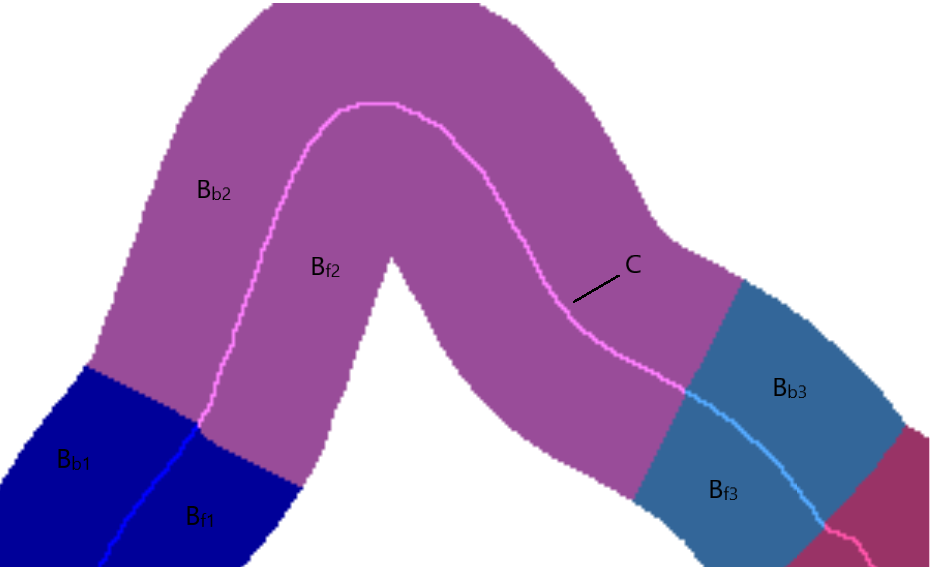
\includegraphics[width=\textwidth]{fig/fb_contour.png}
    \caption{
        Разбиение полосы вокруг контура $\CtLocal$, по которой вычисляется
        функция ошибки, на области $\CtLocalFgI$ и $\CtLocalBgI$
    }
    \label{fig:fb_contour}
\end{figure}

Таким образом, для разбиения полосы достаточно разбить на области точки контура.
Для этого на участки делится поверхность трёхмерной модели объекта: объект
помещается в центр единичной сферы, а сама сфера разбивается на $32$ равные по
площади части по зенитным и азимутным углам.
Каждую точку объекта можно отнормировать, чтобы она попала на поверхность
сферы, и таким образом поделить на области поверхность объекта
(рис.~\ref{fig:color-object-areas}).
Проекция объекта позволяет поделить на области контур
(рис.~\ref{fig:projected-areas}).

\begin{figure}[t]
    \centering
    \begin{minipage}[h]{0.49\linewidth}
        \center{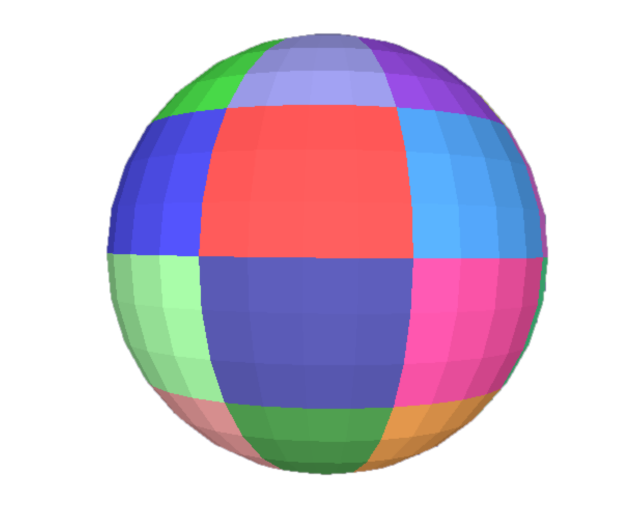
\includegraphics[width=0.8\linewidth]{fig/sphere_straight.png}}
    \end{minipage}
    \hfill
    \begin{minipage}[h]{0.49\linewidth}
        \center{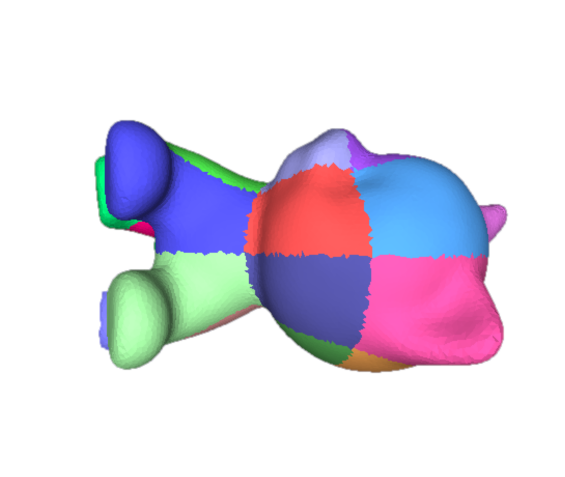
\includegraphics[width=0.8\linewidth]{fig/cat_straight.png}}
    \end{minipage}
    \caption{Разбиение на локальные области поверхностей сферы и объекта}
    \label{fig:color-object-areas}
\end{figure}

\begin{figure}[t]
    \centering
    \begin{minipage}[h]{0.49\linewidth}
        \center{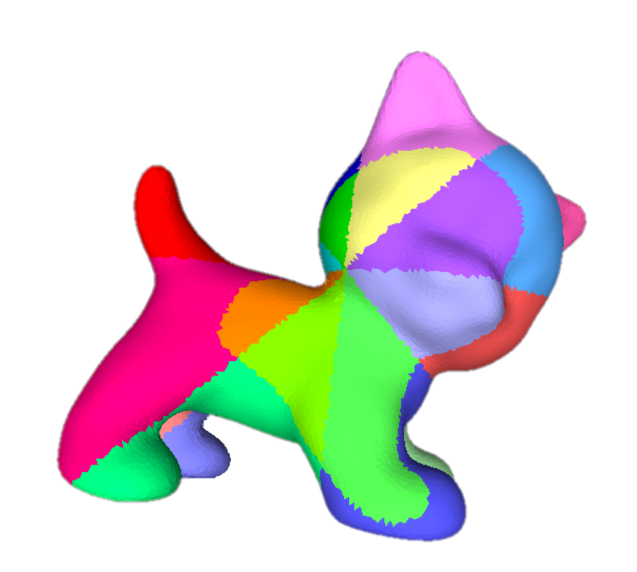
\includegraphics[width=0.8\linewidth]{fig/cat_transformed.png}}
    \end{minipage}
    \hfill
    \begin{minipage}[h]{0.49\linewidth}
        \center{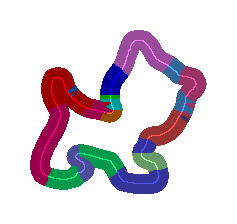
\includegraphics[width=0.8\linewidth]{fig/cat_contour.png}}
    \end{minipage}
    \caption{Слева разбиение на области 3D-модели объекта. Проекция объекта
        разбивает на области контур (правое изображение). Точки вокруг контура
        поппадают в ту же область, что и ближайшие точки на контуре.
    }
    \label{fig:projected-areas}
\end{figure}

Такое разделение объекта неизменно между кадрами, поэтому цветовую информацию
в гистограммах можно накапливать в ходе трекинга.
Данные в гистограммах $\HistLocalFg$ будут при этом отражать распределение
цветов на определённых областях объекта, а данные в гистограммах
$\HistLocalBg$ "--- распределение цветов на фоне вокруг этих областей.
Количество гистограмм не зависит от размера 3D-модели и остаётся небольшим, что
положительно влияет на время работы метода и позволяет обновлять все
гистограммы на каждом кадре.

На локальные области разделяется весь объект целиком.
При этом очевидно, что на отдельном кадре только часть областей будут
спроецированы на контур и поучаствуют в разбиении изображения.
Поэтому информация в некоторых гистограммах может не набираться на протяжении
большого количества кадров.
После поворота объекта такие области могут понадобиться, но информации в
их гистограммах будет недостаточно.

Для решения этой проблемы ведётся учёт \term{опыта} локальных гистограмм и
заводится одна глобальная гистограмма.
Опыт $\ExpLocalI$ локальной пары гистограмм
$\left( \HistLocalFg, \HistLocalBg \right)$
оценивается как общее количество пикселей, попавших
когда-либо в соответсвующую ей область $\CtLocalI$.
Чтобы полученный на старых кадрах опыт учитывался с меньшим весом, чем на
новых, на каждом кадре он домножается на меньший единицы коэффициент:
\begin{equation}
    \ExpLocalI = \CoefFg \ExpLocalINew + (1 - \CoefFg) \ExpLocalIOld
\text{.}
\end{equation}

Если опыт $\ExpLocalI$ меньше некоторого порога $\ExpSuff$,
то вместо значений в локальных гистограммах
$\HistLocalFg$ и $\HistLocalBg$
используются их взвешенные суммы с ячейками глобальных гистограмм
$\HistGlobalFg$ и $\HistGlobalBg$:
\begin{align}\label{eqn:histo_skill}
    \Hf(y) &= \dfrac{\ExpLocalI \HistLocalFg + (\ExpSuff - \ExpLocalI) \HistGlobalFg}{\ExpSuff} \\
    \Hb(y) &= \dfrac{\ExpLocalI \HistLocalBg + (\ExpSuff - \ExpLocalI) \HistGlobalBg}{\ExpSuff}
\text{.}
\end{align}
Порог $\ExpSuff$ выбирается как среднее значение опыта по всем локальным
гистограммам.

\subsection{Комбинирование методов}\label{combining}

Предлагаемый подход комбинирования алгоритмов заключается в их последовательном
применении и инициализации одного метода другим.

Ошибки цветового алгоритма часто бывают вызваны тем, что оптимизация функции
энергии сходится к локальному оптимуму.
Этого можно избежать, если точка инициализации достаточно близка к искомому
глобальному минимуму.
Кроме того, хорошая инициализация позволяет сократить время оптимизации
цветовой функции ошибки и повысить общую производительность метода.
Роль такой инициализации в предлагаемом методе играет результат алгоритма
ключевых точек.

С другой стороны, качество работы алгоритма на основе точечных особенностей
сильно зависит от точности вычисления 3D-прообразов ключевых точек.
Она, в свою очередь, зависит от точности позиции объекта в кадрах, на которых
происходит это вычисление, что ведет к опасности накопления ошибки.
Поэтому предлагается использовать оптимизированные цветовым алгоритмом позиции
объекта для вычисления 3D-прообразов новых ключевых точек и уточнения
прообразов старых.

\newcommand{\XOld}{\ensuremath{\xvec_{\text {\it old}}}}
\newcommand{\XNew}{\ensuremath{\xvec_{\text{\it new}}}}
\newcommand{\ReprErr}[1]{\ensuremath{\vect{e}( #1 )}}

Схема комбинирования алгоритмов показана на рис.~\ref{fig:combining_schema}.

\begin{figure}[t]
    \centering
    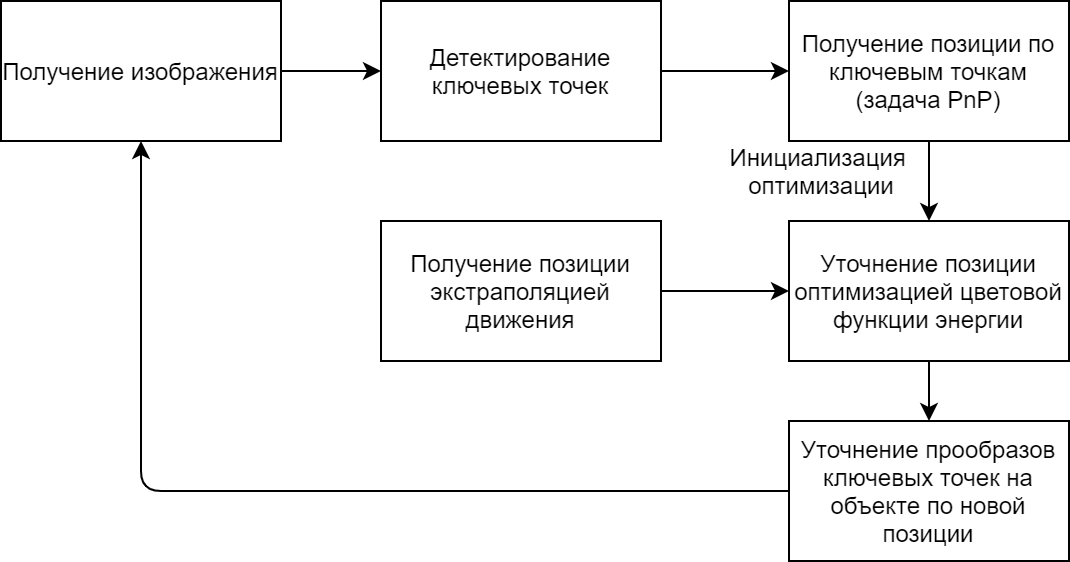
\includegraphics[width=\textwidth]{fig/combining_schema.png}
    \caption{
        Схема комбинирования алгоритмов
    }
    \label{fig:combining_schema}
\end{figure}

На каждом новом кадре позиция объекта сначала вычисляется с помощью
описанного в разделе~\ref{subs:feat_tracking} метода ключевых точек.
При благоприятных условиях данная позиция будет близка к глобальному минимуму
цветовой энергии.
В таком случае выгодно использовать эту позицию как начальную в оптимизации.
Если же метод ключевых точек отработал плохо (например, из-за смазанности
изображения), то такая позиция может оказаться далеко от искомого оптимума и
из нее цветовой алгоритм может не сойтись.
В подобных ситуациях может помочь альтернативный способ вычисления начального
положения, экстраполирующий движение по положениям объекта на двух предыдущих
кадрах.
Из двух возможных начальных позиций для инициализации предлагается выбирать ту,
в которой цветовая функция ошибки покажет меньшее значение.

Оптимизированная цветовым алгоритмом позиция используется в работе с точечными
особенностями.
3D-прообразы обнаруженных впервые ключевых точек строятся уже из этой позиции.
С её помощью также проводится фильтрация выбросов: исключаются из рассмотрения
те 2D-3D-соответствия, для которых ошибка репроекции из уточнённой позиции
больше определённого порога.
Помимо этого, удаляются точки, которые не попадают на передний план, то есть не
лежат на проекции объекта.
Кроме того, при вычислении 3D-прообраза ключевой точки точки запоминается
полигон 3D-модели, на котором он лежит.
Если некоторый полигон не виден на переднем плане, то лежащие на нём точки
считаются невидимыми и тоже далее не рассматриваются.
Таким образом фильтруются 2D-3D соответствия, не согласующиеся с уточненной
цветовым алгоритмом позицией объекта.

Для точек, которые не были отфильтрованы и наблюдались на предыдущих кадрах,
3D-координаты еще раз считаются с использованием оптимизированной позиции
объекта.
Эти новые 3D-координаты ключевой точки заменят старые на следующем кадре, если
будут иметь меньшую ошибку репроекции на изображение.
Пусть $\uvec_{i + 1}$ "--- 2D-координаты точечной особенности на кадре
$\Img_{i + 1}$, а $\xvec$ "--- ее 3D-координаты.
Тогда ошибка репроекции считается как
\begin{equation}\label{eqn:err_reproj}
    \ReprErr{\xvec} = \| \uvec_{i + 1} - \projAt{\Pose_{i + 1}}(\xvec) \|
\end{equation}
Старые 3D-координаты $\XOld$ заменяются на новые $\XNew$, если
$\ReprErr{\XNew} < \ReprErr{\XOld}$.
Сравнивать их сразу же на кадре~$i$ было бы некорректно, так как ошибка
репроекции $\XNew$ на нем нулевая.

Описанные выше действия позволяют согласовать 2D-3D соответствия с уточнённой
позицией.

\section{Скрещивание методов}

\subsection{Последовательное применение алгоритмов}
Первый способ скрещивания алгоритмов заключается в последовательном их применении и инициализации одного метода другим. Метод на основе распределения цветов требует пересчёта большого количества гистограмм и использования их при каждом вычислении функции ошибки и градиента, поэтому является более вычислительно сложным, чем метод ключевых точек, поэтому для скорости трекинга важно сократить количество итераций, за которое он сходится.

Позиции объекта на видео определяются последовательно, от кадра к кадру. Введём обозначения:

$F_{feat}(I)$ -- результат работы алгоритма ключевых точек на изображении $I$; 

$F_{color}(T, I)$ -- результат работы цветового алгоритма на изображении $I$ при инициализации его позицией $T$;

$E_{color}(T)$ -- функция энергии цветового алгоритма от позиции $T$.

Тогда при обработке $i$-ого кадра проводится следующая последовательность действий:

\begin{enumerate}
\item Чтение изображения $I_i$
\item Вычиление позиции алгоритмом ключевых точек: $T_{feat}^{(i)} = F_{feat}(I_i)$
\item Уточнение позиции цветовым методом: $T^{(i)} = F_{color}(T_{feat}, I_i)$
\item Вычисление  3D-позиций, соответствующих ключевым особенностям с использованием позиции $T^i$
\end{enumerate}

После получения изображения проиходит вычисление позиции $T_{feat}$ алгоритмом ключевых точек, описанным в главе 2.2.  Чаще всего эта позиция близка к глобальному минимуму функции энергии цветового алгоритма, но если метод ключевых точек отработал плохо (например из-за смазанности изображения), то эта позиция может оказаться далеко от оптимума, и из-за этого цветовой алгоритм может не сойтись. Чтобы избежать таких случаев, предусмотрен альтернативный способ инициализации позиции. 

Наиболее естественный способ инициализировать алгоритм трекинга при отсутствии специального метода инициализации -- это взять позицию с предыдущего кадра. Но очень часто неправильная работа трекинга на ключевых точках вызвана смазанностью при быстром движении объекта. Чтобы учесть это движение, мы вычисляем альтернативную позицию экстраполяцией движения с предыдущих кадров: $T^{(i)}_{ex} = \Delta T T^{(i - 1)} = T^{(i - 1)}(T^{(i - 2)})^{-1} T^{(i - 1)}$.

Алгоритм цветового трекинга сам выбирает, какую позицию использовать для инициализации. Выбирается та из них, на которой функция энергии цветового алгоритма будет меньше. $T_{color_init} = argmin(E_{color}(T_{feat}), E_{color}(T_{ex}))$.

Чтобы этот выбор не занимал слишком много времени, вычисление $E_{color}$ здесь проводится на 1\% гистограмм.

Для каждой отслеживаемой ключевой особенности известна её 3D-позиция на объекте. Для ключевых особенностей, которые впервые появились на текущем кадре, требуется эту позицию найти. Так как матрица трансформации, полученная цветовым алгоритмом, считается уточнением матрицы, полученной алгоритмом ключевых точек, именно она используется для восстановления 3D-позиций.

\Comment{TODO: процесс восстановления 3D-позиций?}

Для точечных особенностей, которые присутствовали и на предыдущих кадрах, 3D-позиция на объекте известна. Однако то положение объекта, на котором она была вычислена, могло оказаться неверным, и тогда 3D-позиция точки также вычислено неправильно. Эта ошибка сохраняется в течение всего времени, пока данная точечная особенность отслеживается. Чтобы уточнить такие 3D-точки, все они пересчитываются на новом кадре, и если новая позиция оказалась лучше, то она заменяет старую.

Чтобы определить, какая позиция лучше, нужно оценить ошибку репроекции для каждой позиции. Но ошибка репроекции будет нулевой для кадра, по которому позиция вычислена, поэтому нужно выбрать какой-то кадр, на котором обе ошибки будут отличны от нуля. Вопрос об обновлении позиции откладывается до следующего кадра, и решается уже по репроекции на нём. 

Пусть $T_{old}$ - трансформация, на которой была вычислена позиция $X_{old}$, $T_{new}$ - трансформация, на которой была вычислена позиция $X_{new}$, $new > old$.

Пусть $x_0$ - позиция точечной особенности на изображении $new + 1$. 

Тогда $x_{old} = \pi (K (T_{new + 1})_{3 \times 4} X_{old})$

$x_{new} = \pi (K (T_{new + 1})_{3 \times 4} X_{new})$

$e_{old} = \| x_{old} - x_0 \|$

$e_{new} = \| x_{new} - x_0 \|$

При $e_{new} < e_{old}$ позиция $X_{old}$ заменяется на $X_{new}$.

\subsection{Совместная оптимизация}

\section{Эксперименты}\label{experiments}

Предлагаемый в данной работе метод протестирован с помощью открытого набора
данных OPT\cite{OPT}.
Эксперименты проводились на персональном компьютере с процессором Intel Core
i7CPU @ 2.7 GHz.
Данная работа исследует повышение точности трекинга, и предлагаемый алгоритм не
работает в режиме реального времени.
Поэтому сравнение различных модификаций алгоритма, а также сравнение с другими
алгоритмами проводится по точности трекинга.
Кроме того, для некоторых методов, с которыми производится сравнение,
доступны только результаты тестирования без исходного кода.
Различие в используемом для тестирования аппаратном обеспечении не позволяет
корректно сравнивать скорость работы алгоритмов между собой.

\subsection{Данные, используемые для тестирования}

OPT содержит шесть тестовых предметов, для каждого из которых отснято
по 92 видео с разрешением $1920\times1080$.
В каждом кадре известны истинные позиции объектов.
Предметы делятся на три группы по сложности геометрии 3D-моделей: простая
(\term{Soda}, \term{Chest}), средняя (\term{Ironman}, \term{House})
и высокая (\term{Bike}, \term{Jet}).

Видео записаны в различных условиях освещенности, воспроизводят разнообразные
траектории и скорости движения и поделены на следующие группы тестов:
\begin{itemize}
\item \term{$x$-$y$ translation} (\term{Tr}) "--- движение по окружности,
параллельной
        сенсору камеры.
\item \term{$z$ translation} (или \term{zoom}, \term{Zo}) "--- движение вперед
и
        назад вдоль оси, перпендикулярной сенсору камеры.
\item \term{In-plane rotation} (\term{Ir})"--- вращение вокруг оси,
перпендикулярной
        плоскости сенсора камеры.
\item \term{Out-of-plane rotation} (\term{Or})"--- вращение вокруг оси,
параллельной
        плоскости сенсора камеры.
\item \term{Flash light} (\term{Fl})"--- незначительное движение в мигающем
свете.
\item \term{Moving light} (\term{Ml})"--- незначительное движение объекта в
свете значительно
        перемещающегося источника освещения.
    \item \term{Free motion} (\term{Fm})"--- произвольное движение.
\end{itemize}

Группы тестов \term{translation} и \term{rotation} содержат пять различных
уровней скорости.

\subsection{Измерение ошибки}

Ошибка оцененной позиции $\Pose_i$ в кадре $i$ вычисляется как
$
\delta_i = \avg_{\homv{x} \in \MeshV} \norm{\hat{\Pose_i} \homv{x} - \Pose_i
\homv{x}}
$,
где $\MeshV$~--- вершины 3D-модели,
а $\hat{\Pose_i}$ "--- истинная позиция объекта.
Положение объекта считается успешно найденным, если $\delta_i < k d$, где
$d$~--- максимальное из расстояний между всеми парами вершин, а $k$~---
заданный коэффициент ошибки.

Для оценки результатов трекинга строится кривая, каждая точка которой
определяется как процент кадров, на которых успешно определена позиция
объекта, относительно варьируемого параметра $k$.
Чем больше площадь под данной кривой \term{(AUC)}, тем выше эффективность
рассматриваемого решения.
В данной работе берутся значения $k$ от 0 до 0.2.

\subsection{Анализ эффективности отличительных особенностей метода}

Данный раздел посвящен анализу того, как предлагаемые модификации
представленного алгоритма влияют на качество трекинга.
Для тестирования отобрано подмножество набора данных, включающее в себя
наиболее часто встречающиеся на практике паттерны движения.
К ним относятся произвольное движение, а также вращения и параллельные переносы
объекта относительно камеры на скорости $4$ (выше средней).
Эта скорость достаточно высока и приводит к небольшому смазыванию изображений,
что нередко встречается в реальных условиях.
При этом смазывание ещё не слишком сильно и очертания объектов хорошо
различимы.
Также включены примеры с изменяющимся освещением, так как этот фактор негативно
влияет как на цветовой трекинг, так и на трекинг с использованием ключевых
точек.

\subsubsection{Комбинирование цветового и точечного методов}

Текущий подраздел содержит исследование того, насколько комбинирование методов
помогает справляться с неблагоприятными условиями.

Протестированы: метод на основе ключевых точек, метод на основе
распределения цвета и их комбинация.
На рис.~\ref{fig:combining-plots} представлены результаты трекинга этими
методами для разных групп тестов и для всего выбранного подмножества набора
данных.
В табл.~\ref{tab:combine} указаны значения AUC для соответствующих графиков.

\begin{table}[h]
\caption{\label{tab:combine}Результаты комбинирования методов в сравнении с
методами по отдельности}
\begin{center}
\begin{tabular}{|c|c|c|c|c|c|c|c|c|}
\hline
Метод & Общее & Fl & Fm & Ir & Ml & Or & Tr & Zo \\
\hline
Распределение цвета & 7.876 & $6.026$ & $7.757$ & $16.088$ & $5.471$ & $12.963$
&
$10.122$ & $3.743$ \\
\hline
Ключевые точки & 8.804 & $0.717$ & $8.561$ & $15.745$ & $11.248$ & $12.359$ &
$12.55$
&$12.219$ \\
\hline
Комбинация & $\mathbf{12.012}$ & $\mathbf{12.269}$ & $\mathbf{10.039}$ &
$\mathbf{16.932}$ &
$\mathbf{13.345}$ & $\mathbf{12.974}$ & $\mathbf{12.958}$ &
$\mathbf{12.583}$ \\
\hline
\end{tabular}
\end{center}
\end{table}

\begin{figure}
\centering
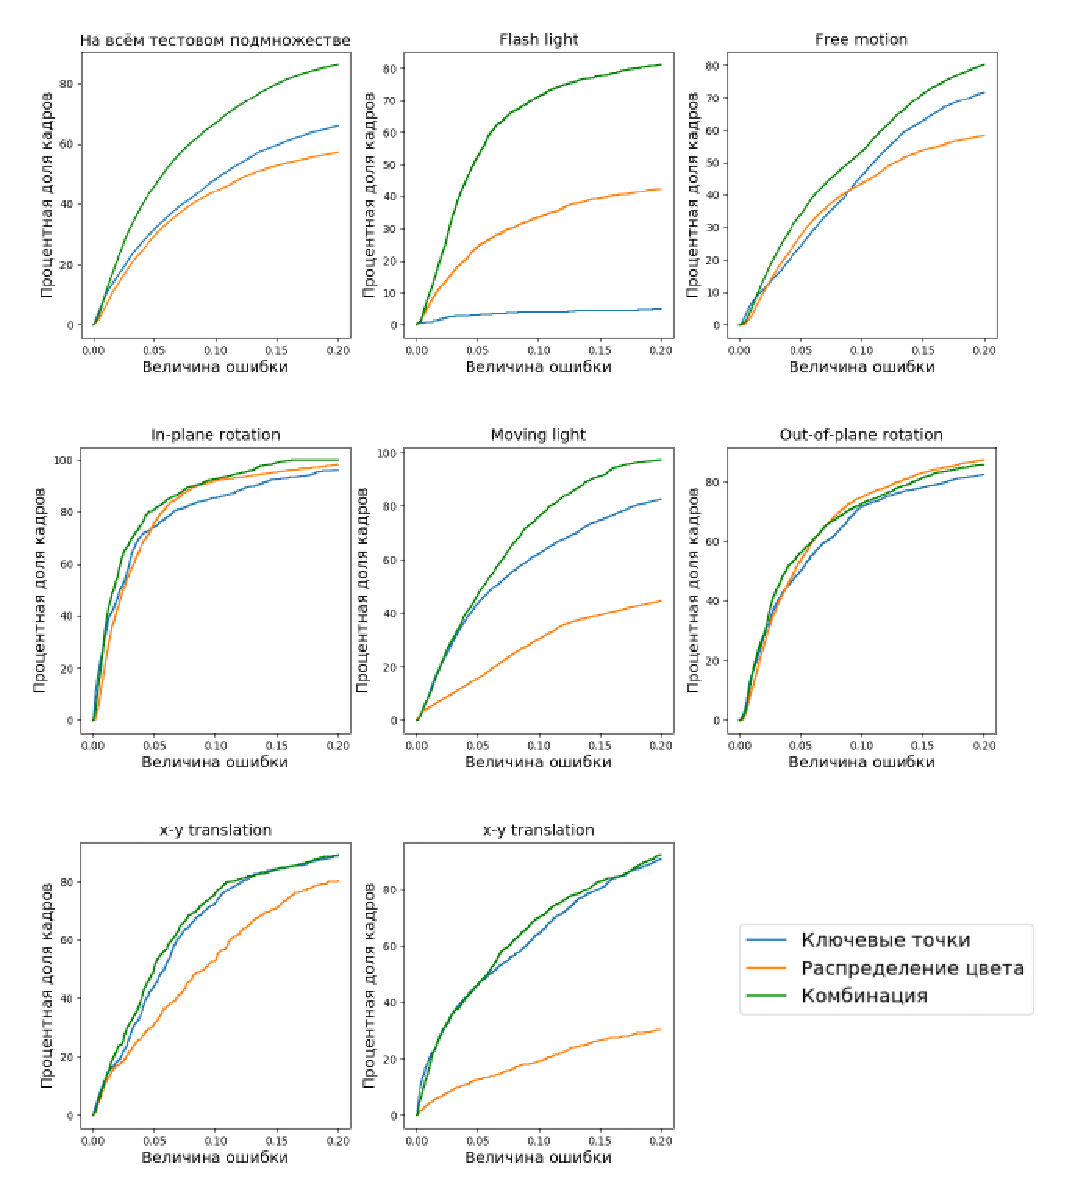
\includegraphics[width=0.9\textwidth]{fig/Combining.pdf}
\caption{
Сравнение точности методов по отдельности и их комбинации на всём подмножестве
датасета и на группах тестов
}
\label{fig:combining-plots}
\end{figure}


Для всех групп комбинированный метод оказался лучше методов по отдельности.
По графику для всего подмножества датасета на рис.~\ref{fig:combining-plots}
можно заметить, что кривая для комбинированного метода почти совпадает с
кривыми для отдельных методов на левом конце и заметно превышает их на правом
конце графика.
Это говорит о том, что при комбинировании не увеличивается количество кадров,
где объект отслеживается почти идеально, но значительно растёт число кадров, на
которых объект отслеживается хотя бы с какой-то приемлемой точностью.

Комбинированный метод точнее отслеживает объект там, где отдельные методы
ошибались слишком сильно.
Таким образом, преимущества комбинирования более явно прослеживаются в сложных
для трекинга условиях.
Инициализация алгоритмом ключевых точек может значительно улучшить точность
цветового метода, что видно на примере группы \term{zoom}.
Это объясняется тем, что цветовой метод инициализируется вблизи глобального
минимума функции энергии, и даже если оптимизация сойдётся к локальному
минимуму, то результат будет недалёк от истинной позиции.

В группе тестов с мигающим светом (\term{Flash light}) оба отдельных метода
испытывают сложности, однако в комбинации удерживают друг друга вблизи
истинной позиции.
Позиция, уточнённая цветовым алгоритмом, помогает отфильтровать неправильно
отслеженные 2D-3D-соответствия.
Для ключевых точек, обнаруженных на кадре впервые, строятся более качественные
3D-прообразы.
Если такие точки будут прослеживаться хотя бы на нескольких кадрах, это во
многих случаях позволит строить по ним хорошую инициализацию цветового
алгоритма.
Такая инициализация, в свою очередь, позволяет оптимизации сойтись гораздо ближе
к истиной позиции. Таким образом, алгоритмы дополняют друг друга и их комбинация
позволят значительно повысить точность каждого по отдельности.

На группах тестов, где результаты отдельных методов не ниже $10$
(\term{In-plane rotation}, \term{Out-of-plane rotation}, \term{$x$-$y$
translation}), комбинация показывает незначительное улучшение, и её результат
примерно соответствует результату лучшего из отдельных методов.
Это тесты с постоянным освещением, где траекторией движения является вращение
или перенос.
На них единственным фактором, негативно влияющим на качество трекинга, является
высокая скорость, и, как следствие, смазанность изображений.
Оба метода сохраняют работоспособность в таких условиях, и дополнение одного
метода другим незначительно увеличивает точность.


\subsubsection{Организация гистограмм}

В данной работе вводится подход к организации гистограмм, ограничивающий их
количество константой.
Он позволяет снизить потребление оперативной памяти, сократить время
обновления гистограмм и вычисления функции энергии.
\Comment{Кратко напомнил, почему это хорошо.}
В то же время это потенциально может ухудшить точность метода в сравнении с
подходом, в котором для каждой вершины используется пара гистограмм.
В табл.~\ref{tab:full_hist} сравниваются два способа реализации
комбинированного алгоритма: в одном из них гистограммы организованы согласно
описанию в главе~\ref{tracking}.
В другом испольузется подход, описанный в~\cite{Tjaden2017}
и~\cite{Tjaden2018}: пара гистограмм строится для каждой вершины и действует в
окрестности её проекции, если эта проекция оказалась вблизи контура.
При тестировании использованы гистограммы всех вершин, спроецированных рядом
с контуром, в отличие от~\cite{Tjaden2017} и~\cite{Tjaden2018}, где выбиралась
только часть таких вершин.
Такой подход позволяет обновлять информацию в большем числе гистограмм и
избавляет от рисков, связанных с неправильным их выбором, хотя и ухудшает
скорость работы.

\begin{table}[h]
\caption{\label{tab:full_hist}Влияние организации гистограмм на точность}
\begin{center}
\begin{tabular}{|c|c|c|c|c|c|c|c|}
\hline
Метод & Fl & Fm & Ir & Ml & Or & Tr & Zo \\
\hline
Пара гистограмм на каждую вершину & $7.27$ & $\mathbf{11.126}$ &
$\mathbf{17.279}$ & $12.302$ & $\mathbf{15.279}$ & $12.529$ &
$\mathbf{13.723}$\\
\hline
32 пары гистограмм & $\mathbf{12.269}$ & $10.039$ & $16.932$ &
$\mathbf{13.345}$ & $12.974$ &
$\mathbf{12.958}$ & $12.583$ \\
\hline
\end{tabular}
\end{center}
\end{table}

Можно заметить, что на большинстве паттернов  точность не уменьшилась, либо
уменьшилась незначительно.
Заметно снижение точности на паттернах \term{Or} и \term{Fm}.
На них объект при движении поворачивается другой, не видимой ранее, стороной, и
начинают использоваться гистограммы, достаточная статистика по которым ещё не
собрана.
Менее плотное распределение гистограмм в этом случае ухудшает результат.

\Comment{Добавить результаты цветового метода?}

\subsubsection{Влияние пересчёта 3D-прообразов ключевых точек}

Позиция, полученная цветовым методом, используется для задания 3D-прообразов
ключевых точек, появившихся на текущем кадре впервые.
Вместе с тем, она используется и для коррекции старых точек, если эта коррекция
уменьшает ошибку репроекции.

Если не обновлять 3D-прообразы старых ключевых точек, то они вычисляются
единожды при первом появлении ключевой точки на видео.
Даже если этот прообраз был найден неточно, он в дальнейшем не обновляется.

В табл.~\ref{tab:reprojection} представлены результаты трекинга с коррекцией
старых 3D-позиций и того же алгоритма, в котором 3D-позиции вычисляются
только при первом появлении ключевой точки и далее не пересчитываются.

\begin{table}[h]
\caption{\label{tab:reprojection}Влияние пересчёта 3D-прообразов}
\begin{center}
\begin{tabular}{|c|c|c|c|c|c|c|c|}
\hline
Метод & Fl & Fm & Ir & Ml & Or & Tr & Zo \\
\hline
Вычисление при первом появлении & $11.209$ & $8.651$ & $16.649$ &
$\mathbf{13.698}$ & $12.788$ & $\mathbf{12.975}$ &
$\mathbf{13.59}$ \\
\hline
С коррекцией старых точек & $\mathbf{12.269}$ & $\mathbf{10.039}$ &
$\mathbf{16.932}$ & $13.345$ &
$\mathbf{12.974}$ &
$12.958$ & $12.583$ \\
\hline
\end{tabular}
\end{center}
\end{table}

Коррекция 3D-позиций в ходе трекинга улучшает точность на группе \term{flash
light}, где алгоритм ключевых точек сам по себе работает плохо.
Также заметно улучшение на группе \term{free motion}, что объясняется
большим разбросом 3D-прообразов одной и той же точки, вычисленных на разных
кадрах.
Это увеличивает вероятность того, что первоначально вычисленный 3D-прообраз
оказался недостаточно точен, но можно будет найти лучший по следующим кадрам.

В группе \term{zoom} трекинг с коррекцией 3D-прообразов менее точен, чем с
однократным их вычислением.
Негативное влияние коррекции здесь связано с 2D-точками, которые
стали отслеживаться неправильно.
Коррекция их 3D-прообразов приводит к тому, что и 3D-позиции смещаются
относительно своего первоначального положения.
<<Неправильное>> 2D-3D-соответствие согласуется, тем не менее, с последней
вычисленной позицией, так как было обновлено в соответствии с ней.
Без репроекции 3D-позиции такое соответствие было бы отфильтровано, и не
оказывало бы в дальнейшем негативного влияния на трекинг.

На остальных группах тестов коррекция 3D-позиций не приводит к значительному
изменению точности трекинга.

%На группе \term{zoom} цветовой трекинг менее точен, чем трекинг на ключевых
%точках.
%В ходе трекинга точность может ухудшаться, поэтому и обновление позиции по
%менее точным кадрам несколько ухудшает результаты.
%На остальных группах пересчёт позиций не улучшает качество трекинга, либо
%улучшает его незначительно.

\Comment{Объяснения пока очень предположительные}

\subsubsection{Сравнение с аналогами}

В табл.~\ref{tab:analogues} представлено сравнение предлагаемого алгоритма с
алгоритмами на основе распределения цвета (PWP3D, RBOT) и комбинированными
алгоритмами (Bugaev et.al., Zhong et.al.).

\begin{itemize}
\item PWP3D "--- один из первых цветовых алгоритмов, в котором использовалась
одна пара гистограмм для всего изображения.
\item RBOT "--- цветовой алгоритм с одной парой гистограмм для каждой вершины
объекта.
\item Bugaev et. al. "--- алгоритм, в котором трекинг на ключевых точках
комбинировался с методом, основанным на контурах. Ключевые точки также
использовались для инициализации трекинга, а затем --- для задания
ограничений при оптимизации контурной функции ошибки.
\item Zhong et.al. "--- алгоритм, в котором отслеживается распределение цвета в
окрестностях контура и градиентные дескрипторы на внутренней части переднего
плана.
\end{itemize}

\begin{table}[h]
\caption{\label{tab:analogues}Сравнение с другими цветовыми и комбинированными
алгоритмами}
\begin{center}
\begin{tabular}{|c|c|c|c|c|c|c|c|}
\hline
Объект & Bike & Chest & House & Ironman & Jet & Soda & Среднее \\
\hline
PWP3D~\cite{PWP3D} & $5.358$ & $5.551$ & $3.575$ &
$3.915$ & $5.813$ & $5.87$ & $5.014$ \\
\hline
RBOT~\cite{Tjaden2018} & $11.903$ & $11.764$ & $10.15$ &
$11.986$ & $13.217$ & $8.861$ & $11.314$ \\
\hline
Bugaev et.al.~\cite{Bugaev_2018_ECCV} & $12.55$ & $14.97$ & $14.48$ &
$\mathbf{14.71}$ & $\mathbf{17.17}$ & $\mathbf{14.85}$ & $\mathbf{14.79}$ \\
\hline
Zhong et.al.~\cite{Zhong2020} & $\mathbf{12.831}$ & $12.24$ & $13.613$ &
$11.214$ & $15.441$ & $9.012$ & $12.392$ \\
\hline
Наш алгоритм & $11.648$ & $\mathbf{15.522}$ & $\mathbf{16.607}$ & $11.556$ &
$13.966$ & $14.104$
& $13.901$ \\
\hline
\end{tabular}
\end{center}
\end{table}

\Comment{Можно как-то выделить еще второе место.}

За счёт локальности RBOT и предлагаемый алгоритм работают значительно лучше PWP3D. 
Наш метод незначительно уступает RBOT на объектах Bike и Ironman. Эти объекты
имеют большое количество вершин и однородную текстуру, в результате чего RBOT
получает преимущество за счёт большего количества гистограмм.
Тем не менее, на тестах Chest, House, Soda c хорошо текстурированными объектами
с невысокой полигональностью инициализация цветового метода
ключевыми точками позволяет существенно превзойти результат RBOT.

Преимущества нашего комбинированного метода явно прослеживаются на объекте Soda.
Этот объект симметричен относительно оси вращения, и цветовой алгоритм
испытывает трудности при его трекинге.
Использование ключевых точек помогает разрешать неоднозначности, связанные с
одинаковым контуром при разных углах поворота объекта вокруг своей оси.

На большей части объектов наш метод превосходит другой комбинированный
метод Zhong et.al., также применяющий цветовую информацию для трекинга.
В том числе значительное улучшение отмечается на симметричном объекте Soda.
При этом результаты нашего метода на объектах с однородной текстурой Bike, Ironman,
Jet отличаются от результатов метода Zhong et.al. несущественно.

На объектах Chest и House предлагаемый метод показывает лучшие результаты, чем
комбиниованный алгоритм Bugaev et.al., но на некоторых объектах (Ironman, Jet)
значительно ему уступает. Тем не менее, в среднем разница в точности небольшая.

Таким образом, предлагаемый в данной статье алгоритм трекинга показывает результаты
на уровне современных комбинированных методов.

\Comment{TODO: больше алгоритмов для сравнения?}
\Comment{TODO: объяснение результатов в сравнении с Bugaev и Zhong?}

\section{Заключение}

\Comment{Вроде выводы ок}

В данной работе рассматривается совмещение трекинга с помощью точечных
особенностей и трекинга на основе распределения цветов.
Предлагаемый алгоритм использует полученную с помощью ключевых точек начальную
позицию для задания отправной точки вычисления окончательной позиции объекта
цветовым методом.
В то же время рассчитанная с помощью цветового метода позиция учитывается при
работе с ключевыми точками и используется для их коррекции.
Преимущества комбинированного алгоритма особенно заметны в сложных для трекинга
условиях.
При этом комбинирование более точного метода с менее точным в целом не ухудшает
его результат.
Взаимная согласованность двух подходов к трекингу позволяет добиваться более
стабильных и качественных результатов, чем с помощью каждого из них по
отдельности, что демонстрируется с помощью экспериментов на открытом тестовом
бенчмарке.


\newpage
\bibliographystyle{plain}
\bibliography{bibliography}
\end{document}

